\documentclass[a4paper,12pt]{extarticle}
\usepackage{Diplo}
\usepackage{subcaption}
%\usepackage{amsmath, amsfonts, amssymb}
%\usepackage[english, russian]{babel}
%\usepackage[utf8]{inputenc}
%\usepackage{graphicx}
%\usepackage{float}
%\usepackage{subfigure}
%\usepackage{color}
%\usepackage{indentfirst}
%\usepackage{hyperref}
%\usepackage{cite}
%\usepackage[noend]{algorithmic}

%\usepackage{geometry}
%\geometry{left=2cm}
%\geometry{right=1.5cm}
%\geometry{top=1cm}
%\geometry{bottom=2cm}

\bibliographystyle{unsrt}

\title{Математические методы диагностики ишемической болезни по электрокардиограмме сверхвысокого разрешения}

\author{И.С.Ямщиков}

\begin{document}

{
\renewcommand{\baselinestretch}{1}
\thispagestyle{empty}
\begin{center}
    \sc
        Министерство образования и науки Российской Федерации\\
        Московский физико-технический институт
        {\rm(государственный университет)}\\
        Факультет управления и прикладной математики\\
        Кафедра <<Интеллектуальные системы>>\\
        при Вычислительном центре им. А. А. Дородницына РАН\\[35mm]

    \rm\large
        Ямщиков Илья Сергеевич\\[10mm]
    \bf\Large
        Математические методы диагностики\\
        ишемической болезни \\
        по электрокардиограмме сверхвысокого разрешения\\[10mm]
    \rm\normalsize
        511656 - Математические и информационные технологии\\[10mm]
    \sc
        Магистерская диссертация\\[30mm]
\end{center}
\hfill\parbox{80mm}{
    \begin{flushleft}
    \bf
        Научный руководитель:\\
    \rm
        д.ф-м.н. Воронцов Константин Вячеславович\\[5cm]
    \end{flushleft}
}
\begin{center}
    Москва\\
    2014 г.
\end{center}
}

\tableofcontents

\newpage
\begin{abstract}
В данной работе исследуется задача ранней диагностики ишемической болезни. Методология базируется на работах сотрудников СПбГМУ и ГУАП по моделированию развития ишемической болезни на крысах. Решается задача классификации ЭКГ на снятые в спокойном состоянии и в ходе развития ишемии по высокочастотным компонентам сигнала. Решается задача поиска участков кардиограммы, построение признаков по которым, позволяет повысить качество классификации. Разработан метод диагностики ишемической болезни по данным ЭКГ высокого разрешения, основанный на локализации амплитудно-частотной характеристики ЭКГ-сигнала. В вычислительном эксперименте показано, что учет локальных особенностей ВЧ части ЭКГ позволяет повысить качество классификации с $75\%$ до $89\%$.
\end{abstract}

\newpage
\section{Введение}

\subsection{ЭКГ}

Электрокардиография\cite{ClinicalECG93}~--- это метод графической регистрации разности потенциалов электрического поля сердца, возникающего при его деятельности. Регистрация производится при помощи аппарата~--- электрокардиографа. Записываемая кривая~--- электрокардиограмма (ЭКГ)~--- отражает динамику в течение сердечного цикла разности потенциалов в двух точках электрического поля сердца, соответствующих местам наложения на теле обследуемого двух электродов.

Сердце обладает такими свойствами как автоматизм - способность сердца самостоятельно вырабатывать импульсы. В наибольшей степени автоматизмом обладает синусовый узел. В нем в покое у здорового человека вырабатывается 60-80 импульсов в минуту. Также сердце обладает свойством возбудимости - оно способно отвечать сокращением на внутренние и внешние раздражители. В норме возбуждения и сокращения сердца возникают под действием импульсов из синусового узла. На рисунке~\ref{fig:ECGSample} приведен пример ЭКГ человека.

\begin{figure}[H]
  \noindent\centering{ 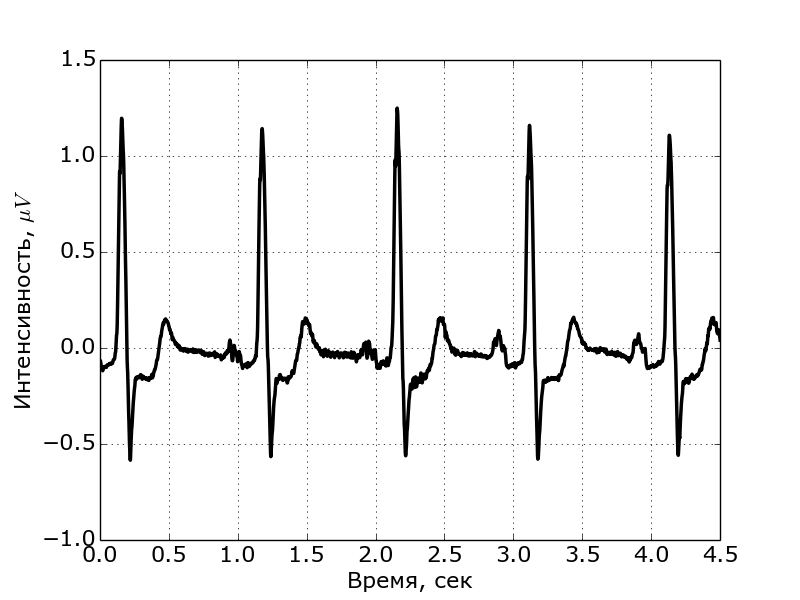
\includegraphics[height = 65mm]{img/sample_ecg.png} }
  \caption{Пример ЭКГ человека.}
  \label{fig:ECGSample}
\end{figure}

Таким образом типичный ЭКГ сигнал имеет периодический характер, связанный с импульсами синусового узла. На ЭКГ обычно выделяют ряд зубцов и интервалов (рисунок~\cite{ECG_ABC03}):

\begin{figure}[h]
  \noindent\centering{ 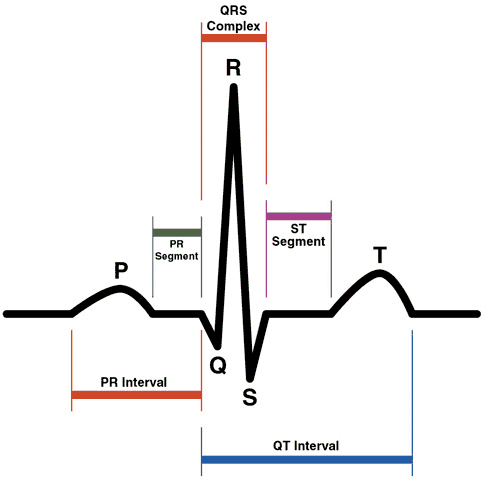
\includegraphics[height = 65mm]{img/ecg_waves.png} }
  \caption{Морфология ЭКГ сигнала}
  \label{fig:ECGWaves}
\end{figure}

\begin{itemize}
    \item P зубец - сумма пиков поочередного возбуждения сначала правого, а затем левого предсердий.
    \item Q зубец - возбуждение межжелудочковой перегородки
    \item R зубец - возбуждение верхушки сердца и прилегающих областей
    \item S зубец - возбуждение основания сердца
    \item T зубец - реполяризация желудочков, восстановление исходного состояния.
\end{itemize}

\subsection{Ишемическая болезнь сердца}

Ишемическая болезнь сердца (ИБС)\cite{IBS06}~--- болезнь, которая развивается при недостаточном поступлении кислорода к сердечной мышце по коронарным артериям. Наиболее частая причина ИБС – атеросклероз коронарных артерий с образованием бляшек и сужением их просвета. В развитых странах ишемическая болезнь сердца стала самой частой причиной смерти и инвалидности — на ее долю приходится около 30 процентов смертности. Она намного опережает другие заболевания в качестве причины внезапной смерти и встречается у каждой третьей женщины и у половины мужчин.

В основе лечения острого коронарного синдрома (обострение стабильного течения ИБС) лежит экстренное восстановление кровотока к сердечной мышце с помощью различных методик. Однако, для выполнения подобных процедур требуется не менее срочная верификация диагноза инфаркта миокарда. В настоящее время диагноз устанавливается на основе клинических, биохимических и электрокардиографических критериев. При этом текущие практические методики диагностики острой ишемии миокарда по ЭКГ-критериям ограничивается алгоритмом <<да-нет>> и лишь приблизительным суждением об очаге поражения миокарда\cite{EIoA_GZ13}.

Актуальной задачей является поиск параметров ЭКГ, коррелирующих с объемом ишемии и ее выраженностью. При этом основной критерий диагностики ишемии~--- девиация сегмента ST~--- не всегда четко коррелирует с ее выраженностью.

\section{Работы проф. К.В. Зайченко и его научной школы}

Авторский коллектив научной школы <<Радиоэлектронные и информационные средства оценки физиологических параметров живых систем>> под руководством проф. К.В. Зайченко решает задачу выявления скрытой информации о патофизиологии благодаря исследованиям тонкой структуры биоэлектрической активности клеток, тканей, органов и систем живых организмов в расширенном амплитудно-частотном диапазоне.

В последнее годы коллективом был разработан метод электрокардиографии сверхвысокого разрешения на основе расширения исследуемых амплитудно-частотных диапазонов электрокардиосигналов.

\subsection{ЭКГ сверхвысокого разрешения}

%С развитием техники повышаются возможности по съему ЭКГ. Развитие современных методов и средств ЭКГ отразилось на:

С общим развитием науки и техники развиваются методы и средства электрокардиографии. Сегодняшней тенденцией является повышение информативности регистрируемых сигналов. В развитии ЭКГ это отразилось, прежде всего, в повышении ее разрешающей способности и характеризуется:

\begin{itemize}
    \item расширением амплитудного и частотных диапазонов регистрации электрокардиосигналов (ЭКС)
    \item использованием различных методов их обработки
    \item автоматизацией анализа ЭКГ
    \item увеличением числа отведений
\end{itemize}

Можно выделить следующие методы повышения разрешающей способности ЭКС:
\begin{itemize}
    \item Крупномасштабная электрокардиография~--- попытка выявления и анализа низкоамплитудных элементов ЭКС. В ней используются технические решения, позволяющие перейти от стандартной чувствительности кардиографа 10мм на 1мВ к повышенной до 50см и более на 1мВ.
    \item Высокочастотная электрокардиография~--- регистрация, выделение и анализ только высокочастотных компонентов ЭКГ в частотном диапазоне более 150Гц
\end{itemize}

Следствием разработок по преодолению недостатков этих методов и стремления к дальнейшему развитию тенденции повышения разрешающей способности средств анализа ЭКГ стало появление нового метода~--- \textit{электрокардиографии сверхвысокого разрешения} (ЭКГ СВР) это был результат более чем двадцатилетней работы коллектива ведущей научной школы <<Радиоэлектронные и информационные средства оценки физиологических параметров живых систем>>. Метод ЭКГ СВР обеспечивает регистрацию ЭКГ на всей протяженности кардиоцикла в более широких амплитудном и частотном диапазонах в условиях воздействия помех. Минимальная граница амплитудного диапазона составляет порядка 10нВ, а максимальная верхняя граница частотного диапазона - более 2000Гц\cite{ECGSR13}.

\subsection{Эксперименты на крысах по моделированию ишемии}

С 2010 года коллективом сотрудников кафедры медицинской радиоэлектроники ГУАП, кафедры патофизиологии Санкт-Петербургского государственного медицинского университета им. акад. И.П.~Павлова и Института экспериментальной медицины Федерального Центра сердца, крови и эндокринологии им. В.А.~Алмазова проводятся совместные исследования по поиску новых ЭКГ-маркеров процесса развития ишемического повреждения миокарда у подопытных животных\cite{EIoA_GZ13}.

Исследования проводились специальных лабораторных макетах, реализующих метод электрокардиографии сверхвысокого разрешения для регистрации низкоамплитудных и высокочастотных составляющих электрокардиосигналов в расширенных амплитудном и частотном диапазонах.

При этом в процессе развития ишемии были зафиксированы значительные изменения компонентов спектра в высокочастотном канале. С развитием ишемии спектральная плотность мощности высокочастотных составляющих ЭКС существенно снижается. И при этом на первой минуте после перевязки левой коронарной артерии, когда процесс развития ишемии уже начался, в ЭКС на выходе низкочастотного канала отсутствуют видимые изменения сигналов по сравнению с нормой, а анализ высокочастотных составляющих уже фиксирует заметное снижение уровня спектральной плотности мощности высокочастотных компонент сигнала ЭКС.

\begin{figure}[H]
    \centering
    \begin{subfigure}[b]{0.31\textwidth}
       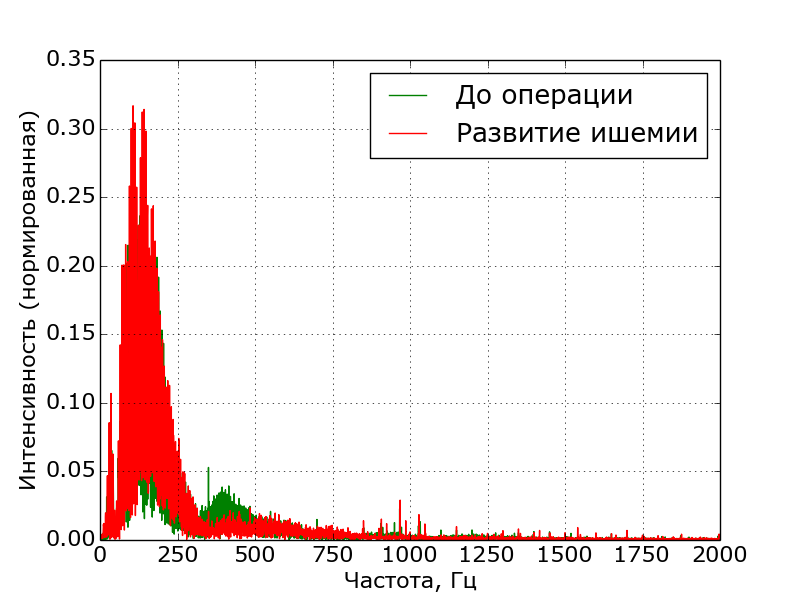
\includegraphics[width=\textwidth]{img/ft_comparison_mouse_1.png}
    \end{subfigure}
    ~
    \begin{subfigure}[b]{0.31\textwidth}
       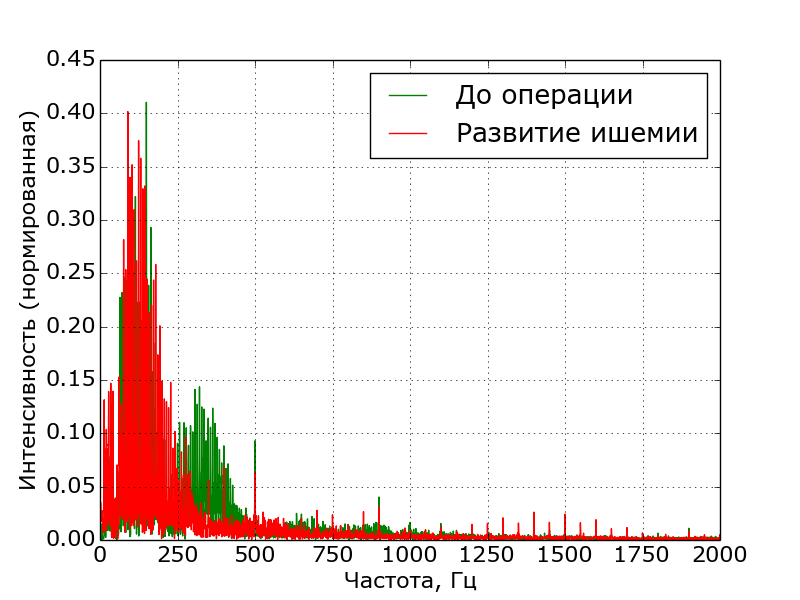
\includegraphics[width=\textwidth]{img/ft_comparison_mouse_16.png}
    \end{subfigure}
    ~
    \begin{subfigure}[b]{0.31\textwidth}
      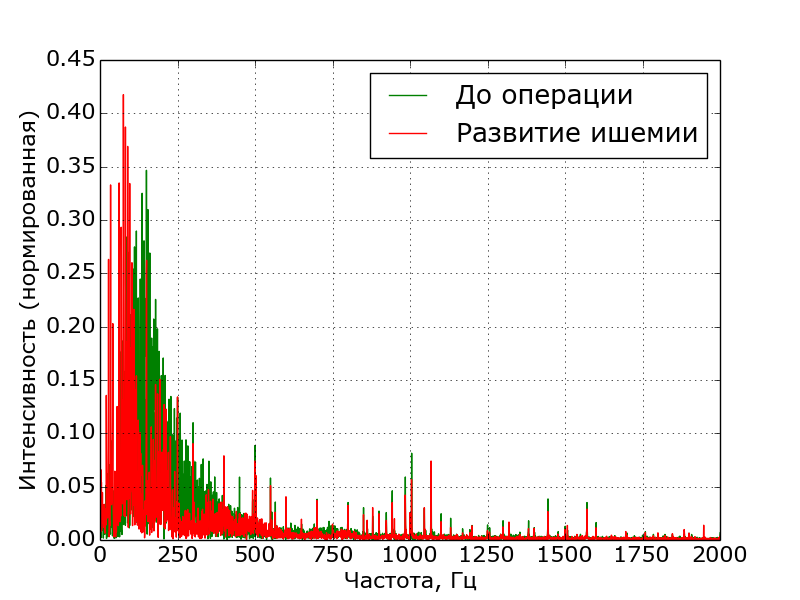
\includegraphics[width=\textwidth]{img/ft_comparison_mouse_3.png}
    \end{subfigure}
    \caption{Сравнение спектров записей до и во время операции для трех различных особей}\label{fig:FTComparison}
\end{figure}

\section{Предлагаемая методика}

Ставится задача классификации ЭКГ на снятые в спокойном состоянии и в ходе развития ишемии по высокочастотным компонентам сигнала.
Пусть имеется набор записей ЭКГ $ECG = \{ecg_i(t)\}_{i=1}^N$. Каждая из них относится к одному из двух классов - ЭКГ снятая до операции либо ЭКГ снятая в процессе развития ишемии. Требуется построить алгоритм, способный классифицировать произвольную ЭКГ.

\subsection{Оценка АЧХ всего сигнала}
\label{ssec:WholeSignalFeaturesTheory}
Построим признаки на основе анализа спектра всего сигнала.

Пусть у нас имеется сигнал ЭКГ: $ecg(t),\; t\in [0,T]$. 

Абсолютная величина сигнала ЭКГ существенно зависит от настроек аппаратуры и может вносить нежелательные искажения, поэтому здесь и в дальнейшем будем рассматривать нормированный сигнал:

$$ \widetilde{ecg} = \frac{ecg}{(\|ecg\|_2)^2} $$

Возьмем преобразование Фурье этого сигнала:

$$f(\omega) = \int\limits_{-\infty}^{\infty} \widehat{ecg}(t)\, e^{-\imath t \omega} dt$$

Отметим, что так как сигнал нормирован, то из равенства Парсеваля следует, что:

$$ \int\limits_{-\infty}^{\infty} |f(\omega)|^2 d\omega =\int\limits_{-\infty}^{\infty} |\widehat{ecg}(t)|^2 dt = 1$$
Таким образом интенсивность фурье-образа так же не зависит от настроек аппаратуры.

В качестве признаков берутся функции от Фурье-образа сигнала. В данной работе были взяты $L2$ нормы отрезков Фурье-образа:
$$ F_[\omega_1, \omega_2] = \int\limits_{\omega_1}^{\omega_2} |\widehat{f}(\omega)|^2 d\omega $$

Например, в качестве системы признаков можно взять разбиение рассматриваемого интервала (0-2000Гц) на $n$ равных отрезков.

\subsection{Учет локальных особенностей АЧХ сигнала ЭКГ}

Следующим шагом является выделение локальных особенностей АЧХ сигнала. На ЭКГ выделяют различные участки - пики, сегменты. И хотелось бы построить признаковое описание электрокардиограммы, используя плотность спектра только на каком-то отдельном участке, например на QRS комплексе.

Для решения этой задачи необходимо разбить сигнал на кардиоциклы.

\subsubsection{Вейвлет-анализ}

Вкратце рассмотрим основные свойства вейвлет преобразования\cite{IntroWavelet03,WaveExampl10}.

Вейвлет-преобразование является важным направлением в технике обработки сигналов, изображений и временных рядов. Сам термин \textit{вейвлет} ввели Гроссманн и Морле в своей статье, посвященной анализу свойств сейсмических и акустических сигналов. Вейвлеты представляют собой особые функции в виде коротких волн с нулевым интегральным значением и локализацией по оси независимой переменной и способных к сдвигу по этой оси и масштабированию. В случае вейвлет-анализа сигнала вейвлеты способны выявить различие в характеристиках процессов на различных шкалах, а посредством сдвига можно проанализировать свойства процесса в различных точках на всем исследуемом интервале.

Вейвлет-преобразование одномерного сигнала - это его представление в виде обобщенного ряда или интеграла Фурье по системе базисных функций

$$ \psi_{ab}(t) =\frac{1}{\sqrt{a}} \psi(\frac{t-b}{a}) $$

сконструированных из исходного (материнского) вейвлета $\psi(t)$ за счет операций сдвига во времени и изменения масштаба.

В качестве материнского вейвлета используется любая функция, удовлетворяющая следующим ограничениям:
\begin{enumerate}
    \item Ограниченность:
        $$ \|\psi\|^2 = \int\limits_{-\infty}^{\infty} |\psi(t)|^2 dt < \infty $$
    \item Нулевое среднее:
        $$ \int\limits_{-\infty}^{\infty} \psi(t) dt = 0 $$
    \item Локализация:
        $ |\psi(t)| \leq C(1+|t|)^{-1-\varepsilon} $ или $ |\widetilde{\psi}(\omega)| \leq C(1+|t|)^{-1-\varepsilon} $
\end{enumerate}

Пример вейвлет функции, использующейся в данной работе, - так называемый вейвлет MHAT. Он задается уравнением

$$ \psi(t) = (1-t^2) e^{-\frac{t^2}{2}} $$

\begin{figure}[H]
  \noindent\centering{ 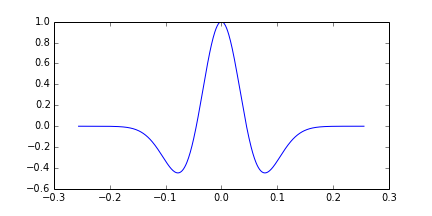
\includegraphics[height = 55mm]{img/ricker_wavelet.png} }
  \caption{MHAT вейвлет}
  \label{fig:MHATWavelet}
\end{figure}

\subsubsection{Непрерывное вейвлет-преобразование.}

Сконструируем базис $\psi_{ab}(t)$ с помощью непрерывных масштабных преобразований и переносов материнского вейвлета с произвольными значениями $a$ и $b$ тогда по определению непрерывное вейвлет преобразование сигнала $f(t)$ запишется:

$$ T(a,b) = \frac{1}{\sqrt{a}} \int\limits_{-\infty}^{\infty} f(t) \psi(\frac{t-b}{a}) dt $$

Таким образом, в отличие от фурье-спектра, вейвлет-спектр является функцией двух аргументов. Первый аргумент $a$ - временной масштаб, аналогичен периоду, т.е. обратен частоте, а второй $b$ - аналогичен смещению сигнала по оси времени.

Также для вейвлет-преобразования существует аналог равенства Парсеваля:

$$ \int\limits_{-\infty}^{\infty} |f(t)|^2 dt = \int\limits_{-\infty}^{\infty} \int\limits_{-\infty}^{\infty} |T(a,b)|^2 \frac{da db}{a^2} $$

\subsubsection{Выделение R пиков}
\label{sssec:RPeaksDetectionTheory}
Рассмотрим задачу разбиения ЭКГ на отдельные кардиоциклы. В существующей литературе описано множество различных подходов к решению этой задачи\cite{Kohler2002}. Приведем основные:

\begin{itemize}
    \item Метода основанные на рассмотрении производных сигнала и различных фильтрах
    \item Подход использующий вейвлет-преобразование сигнала
    \item Использование нейронных сетей
    \item Так же существует множество других подходов, основанных на адаптивных фильтрах, скрытых марковских моделях, морфологии сигнала, генетических алгоритмах, преобразовании Гильберта и т.д.
\end{itemize}

В данной работе был выбран подход с использованием вейвлет-преобразования. А именно алгоритм описанный в~\cite{Chen2009,ApplWTTWave04}. Де-факто стандартной базой данных для оценки алгоритмов выделения R пиков является база MIT-BIH\cite{PhysioNet}. Точность выделения R пиков на этой базе данных у авторов алгоритма составила порядка $99\%$.

Алгоритм:


\textbf{ВХОД:} сигнал $ECG$, масштаб $S$, пороговое значение $H$


\textbf{ВЫХОД:} времена R-пиков кардиоциклов $T_R$
\begin{enumerate}
    \item Вычислить вейвлет-преобразование сигнала $ECG$ с масштабом $S$, используя вейвлет MHAT:
    $$ wt_{S}(t) := \int\limits_{-\infty}^{\infty} ecg(\tau) \psi^*(\frac{\tau-t}{S})d\tau$$
    \item Найти времена, соответствующие локальным максимумам $wt_{S}(t)$
    $$ T_M := \{t_M \in [0, T]: wt_{S}(t_M) - \text{локальный максимум}\} $$
    \item Оставить только пики, с амплитудой выше пороговой:
    $$ T_R := \{t_M \in T_M: wt_{S}(t_M) > H\} $$
\end{enumerate}

Основные достоинства алгоритма:
\begin{itemize}
    \item Устойчивость к шуму. Вейвлет-преобразование сигнала с заданным коэффициентом масштаба очищено как от низкочастотных шумов с характерными периодами больше одного кардиоцикла, так и от высокочастотных шумов.
    \item Хорошее выделение именно R пика. Так как различные пики в сигнале ЭКГ имеют различные масштабы, то возможно настроить данный метод так, чтобы он выделял именно R пики на сигнале.
\end{itemize}

\subsubsection{Локальное выделение признаков}
\label{sssec:LocalFeaturesTheory}
На предыдущем этапе сигнал ЭКГ был разбит на отдельные кардиоциклы, то есть был получен набор отсчетов, соответствующих R пикам сигнала ЭКГ $\{t_{R_i}\}_{i=1}^{N_R}$. Далее вычисляется средняя длина кардиоцикла $\Delta T_R = \left< t_{R_i} - t_{R_{i-1}} \right>$. Для каждого R пика строится окно, заданное параметрами ширины $\Delta w > 0$ и центра $w_0 \in [0;1]$:

$$ \Delta \tau_i = [t_{R_i} + \Delta T_R(w_0 - \frac{\Delta w}{2}); t_{R_i} + \Delta T_R(w_0 + \frac{\Delta w}{2})] $$

При такой параметризации положения окна ширина $\Delta w$ является безразмерной единицей. Характерным интервалом является $\Delta w \in [0; 1]$. При ширине окна большей единицы в его носитель попадут уже несколько кардиоциклов, что не соответствует идее поиска локальных особенностей на участках кардиоцикла. Центр окна $w_0$ так же является безразмерной величиной, нулю соответствует окно с центром в R пике.

Признаки строятся на на основе оконного преобразования Фурье.
$$\widehat{f}_i(\omega) = \int\limits_{-\infty}^{\infty} \widehat{ecg}(t)\,W_{\Delta \tau_i}(t)\, e^{-\imath t \omega} dt$$
Здесь $W(t)$ - оконная функция. В данной работе использовалось окно Хэмминга.

Следует отметить, что в отличие от преобразования Фурье по всему сигналу, оконное преобразование Фурье имеет определенную разрешающую способность по частоте. Так, например, спектр гармонического сигнала будет представлять собой функцию вида $\frac{\sin(x)}{x}$ с лепестками, ширина которых зависит от ширины окна $T$ как $\Delta \omega = \alpha \frac{2\pi}{T}$. Где $\alpha$ является параметром окна.

Так для окна Хэмминга $\alpha=1.333$ и, например, у окна шириной в $0.15$ секунды (длина кардиоцикла у крысы\cite{BioModel2004}) ширина главного лепестка гармонического сигнала будет порядка $50$Гц. Соответственно, два гармонических сигнала с частотами отличающимися менее чем на 50Гц будут неразличимы в Фурье-образе. 

В качестве признаков возьмем, аналогично предыдущему построению системы признаков:
$$ Fw_{\Delta w, w_0}[\omega_1,\omega_2] = \sum_i^N \int\limits_{\omega_1}^{\omega_2} |f_i(\omega)|^2 d\omega ,\quad {t_R}_i \in [1;N_R] $$
Здесь сумма берется по R пикам кардиограммы.

\section{Данные}

Для проверки методики использовалась база данных ЭКГ СПбГМУ им. акад. И.П. Павлова\cite{EIoA_GZ13}, полученная в ходе моделирования ишемии миокарда на крысах. В процессе снимались показания электрокардиографа. Имеются данные по 20 крысам - короткие записи (порядка 2 секунд), снимаемые в отдельные моменты операции: до операции, после вскрытия, в процессе развития ишемии с 1 по 45 минуту примерно по 6 записей для каждой особи (времена съема и количество записей в процессе развития ишемии различно для различных особей). При этом запись велась отдельно по двум каналам - низкочастотном 0.05-100Гц и высокочастотном 100-2000Гц. Более подробно схема описана в \cite{AnalogProcess_Z2009}.

\vspace{0.3cm}

Примеры записей:
\begin{figure}[H]
    \noindent\centering{ 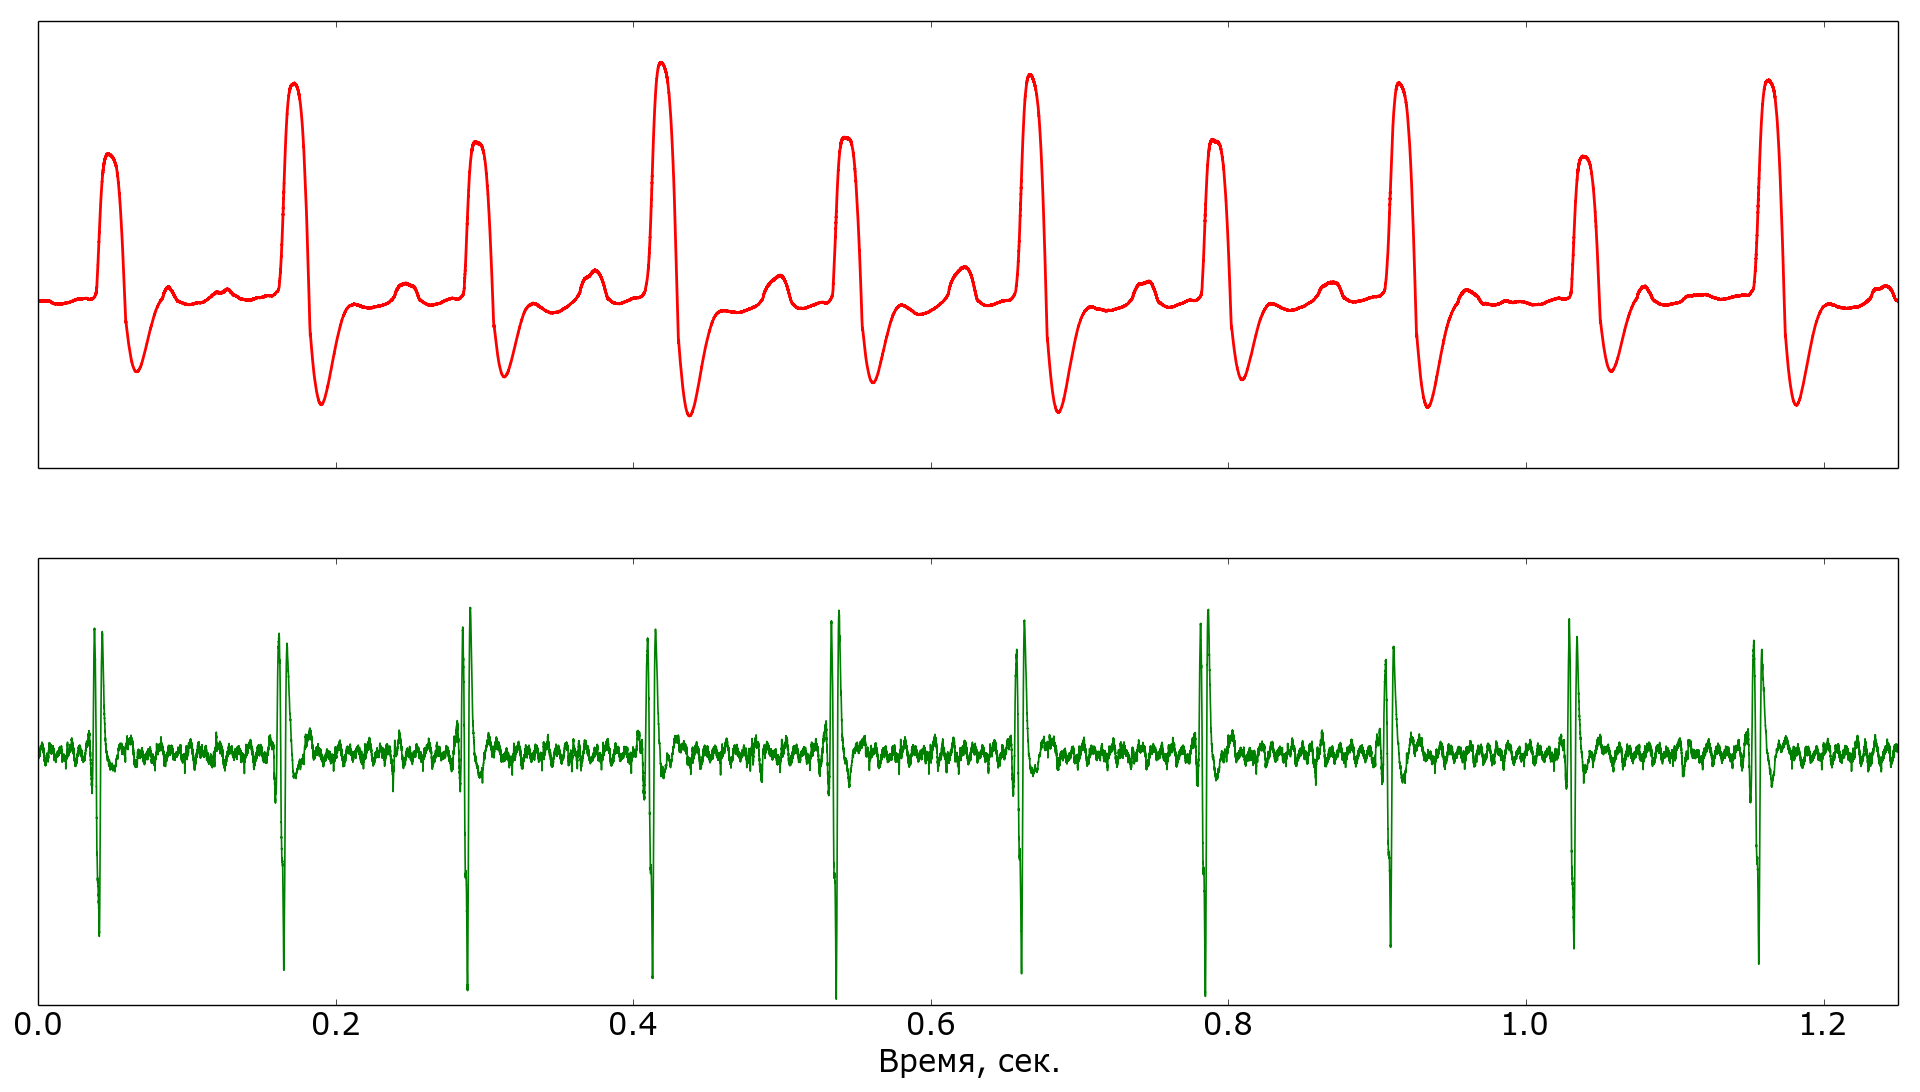
\includegraphics[height = 80mm]{img/record_5_1_high_n_low.png} }
    \caption{Пример электрокардиограммы, снятой до операции. Сверху - низкочастотный канал, снизу высокочастотный}
\end{figure}

\begin{figure}[H]
  \noindent\centering{ 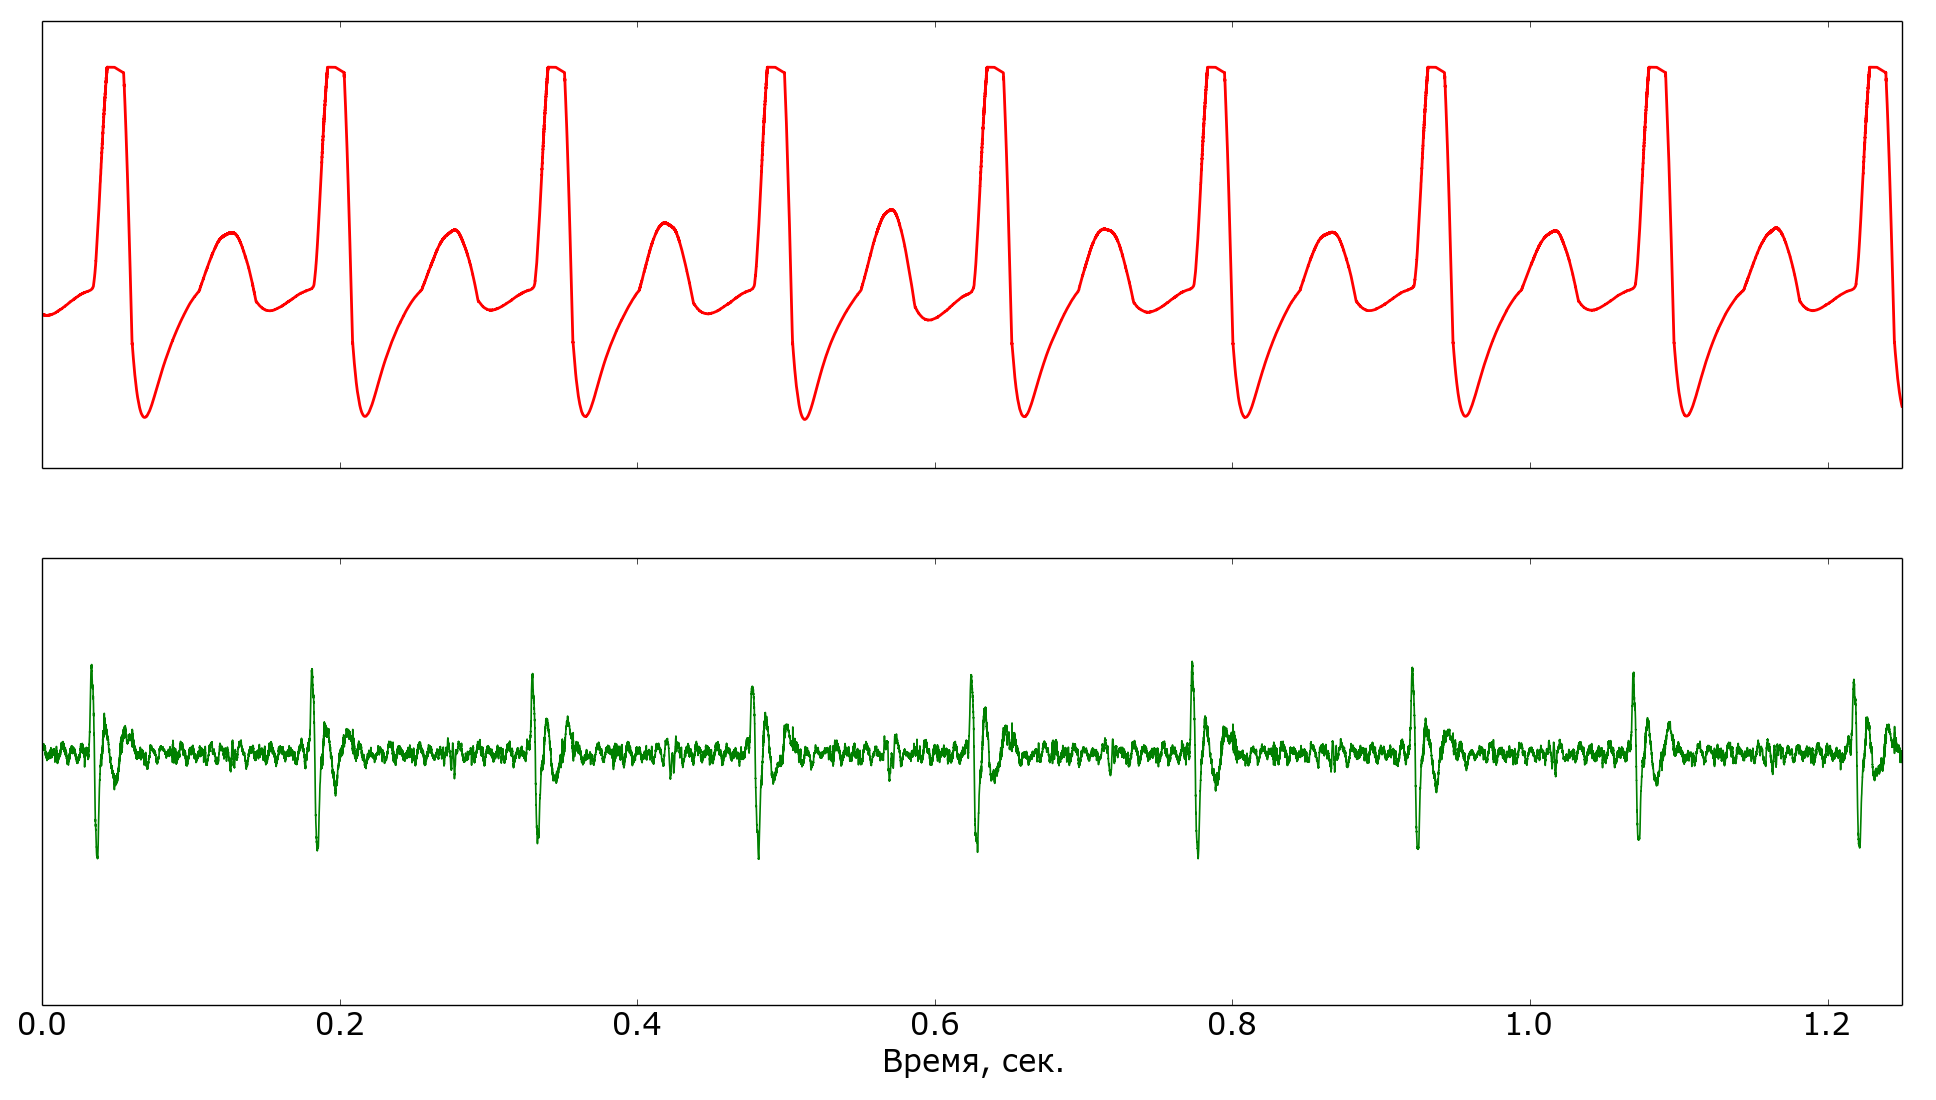
\includegraphics[height = 80mm]{img/record_5_4_high_n_low.png} }
  \caption{ЭКГ снятая на 5 минуте развития ишемии. Сверху - в стандартном частотном диапазоне, снизу высокочастотная часть.}
\end{figure}

Пример спектра высокочастотного канала:

\begin{figure}[H]
  \noindent\centering{ 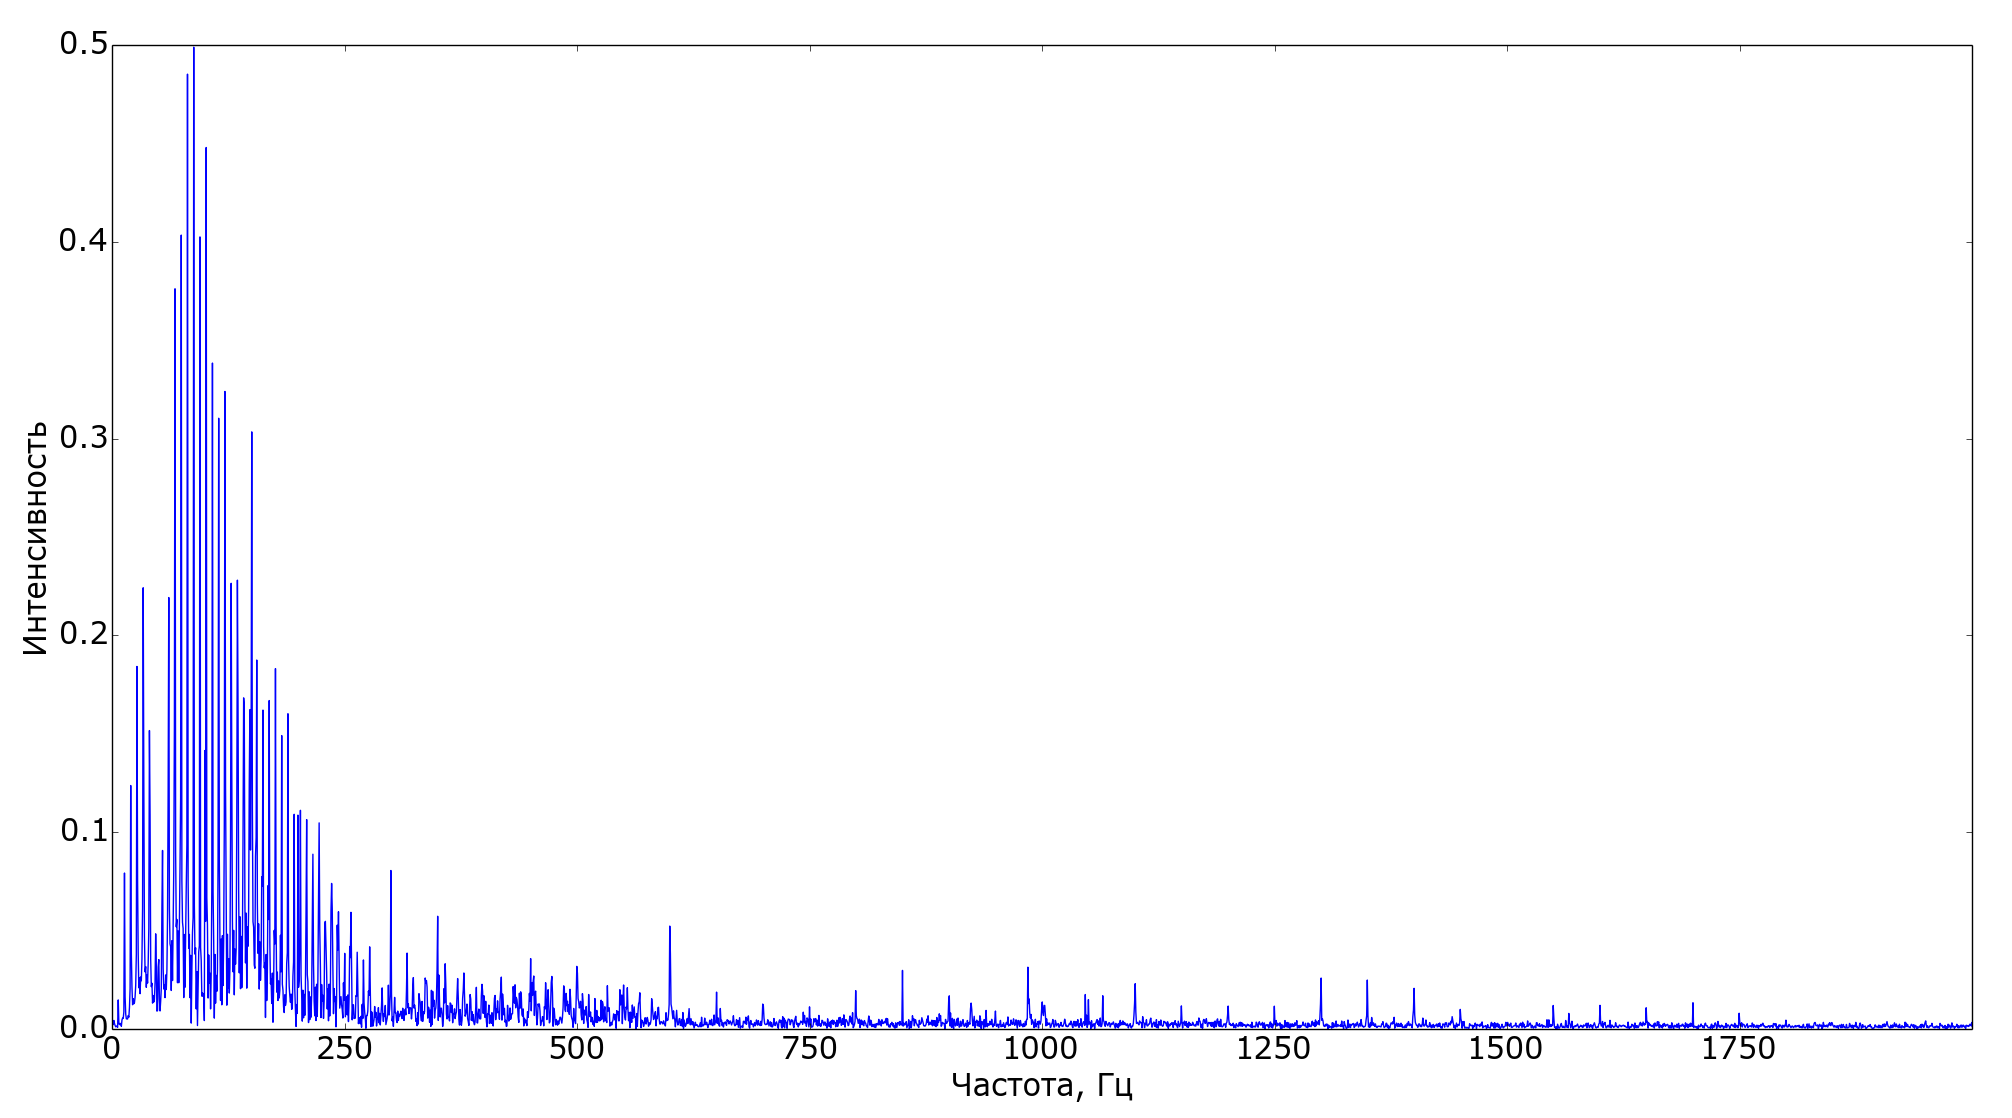
\includegraphics[height = 80mm]{img/record_5_4_fft.png} }
  \caption{Спектр высокочастотной ЭКГ снятой на 5 минуте развития ишемии}
\end{figure}

\section{Эксперименты}

В данном разделе на основе приведенной выше методологии строятся признаковые описания сигналов ЭКГ и исследуются оценки качества классификации по этим признакам.

Основной метрикой качества в данной работе является оценка $5\times5 fold$ кросс-валидации классификатора SVM с линейным ядром.

\subsection{Выделение признаков по спектральным характеристикам всего сигнала}

Рассматривается система признаков, введенная в~\ref{ssec:WholeSignalFeaturesTheory} $\{F[\omega_{i},\omega_{i+1}]\}_{i=1}^{N-1}$, где $\omega_i$ - набор частот, разбивающий исследуемый спектр на множество частотных отрезков. 

Для заданного интервала частот $[\Omega_0, \Omega_1]$ строится набор частот $\omega_i = \Omega_0 +  \frac{i}{N} (\Omega_1 - \Omega_0)$.

Построим признаковое описание ЭКГ с $[\Omega_0, \Omega_1] = [25, 1000]$, $N=10$.

Полученная оценка $5\times5 fold$ кросс-валидации SVM - $75.7\%$

\begin{figure}[H]
    \begin{center}
       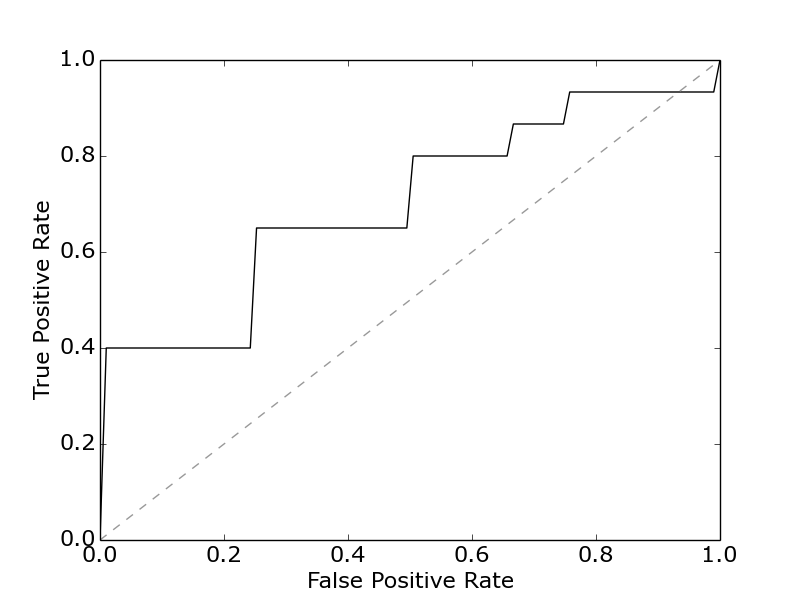
\includegraphics[width=75mm]{img/old_roc.png}
    \end{center}
    \caption{ROC кривая}
\end{figure}

\subsection{Выделение кардиоциклов}

Применим алгоритм, описанный в~\ref{sssec:RPeaksDetectionTheory}.
Параметр алгорима - коэффициент масштаба берется равным $S = 0.004$ секунды.

\begin{figure}[H]
  \noindent\centering{ 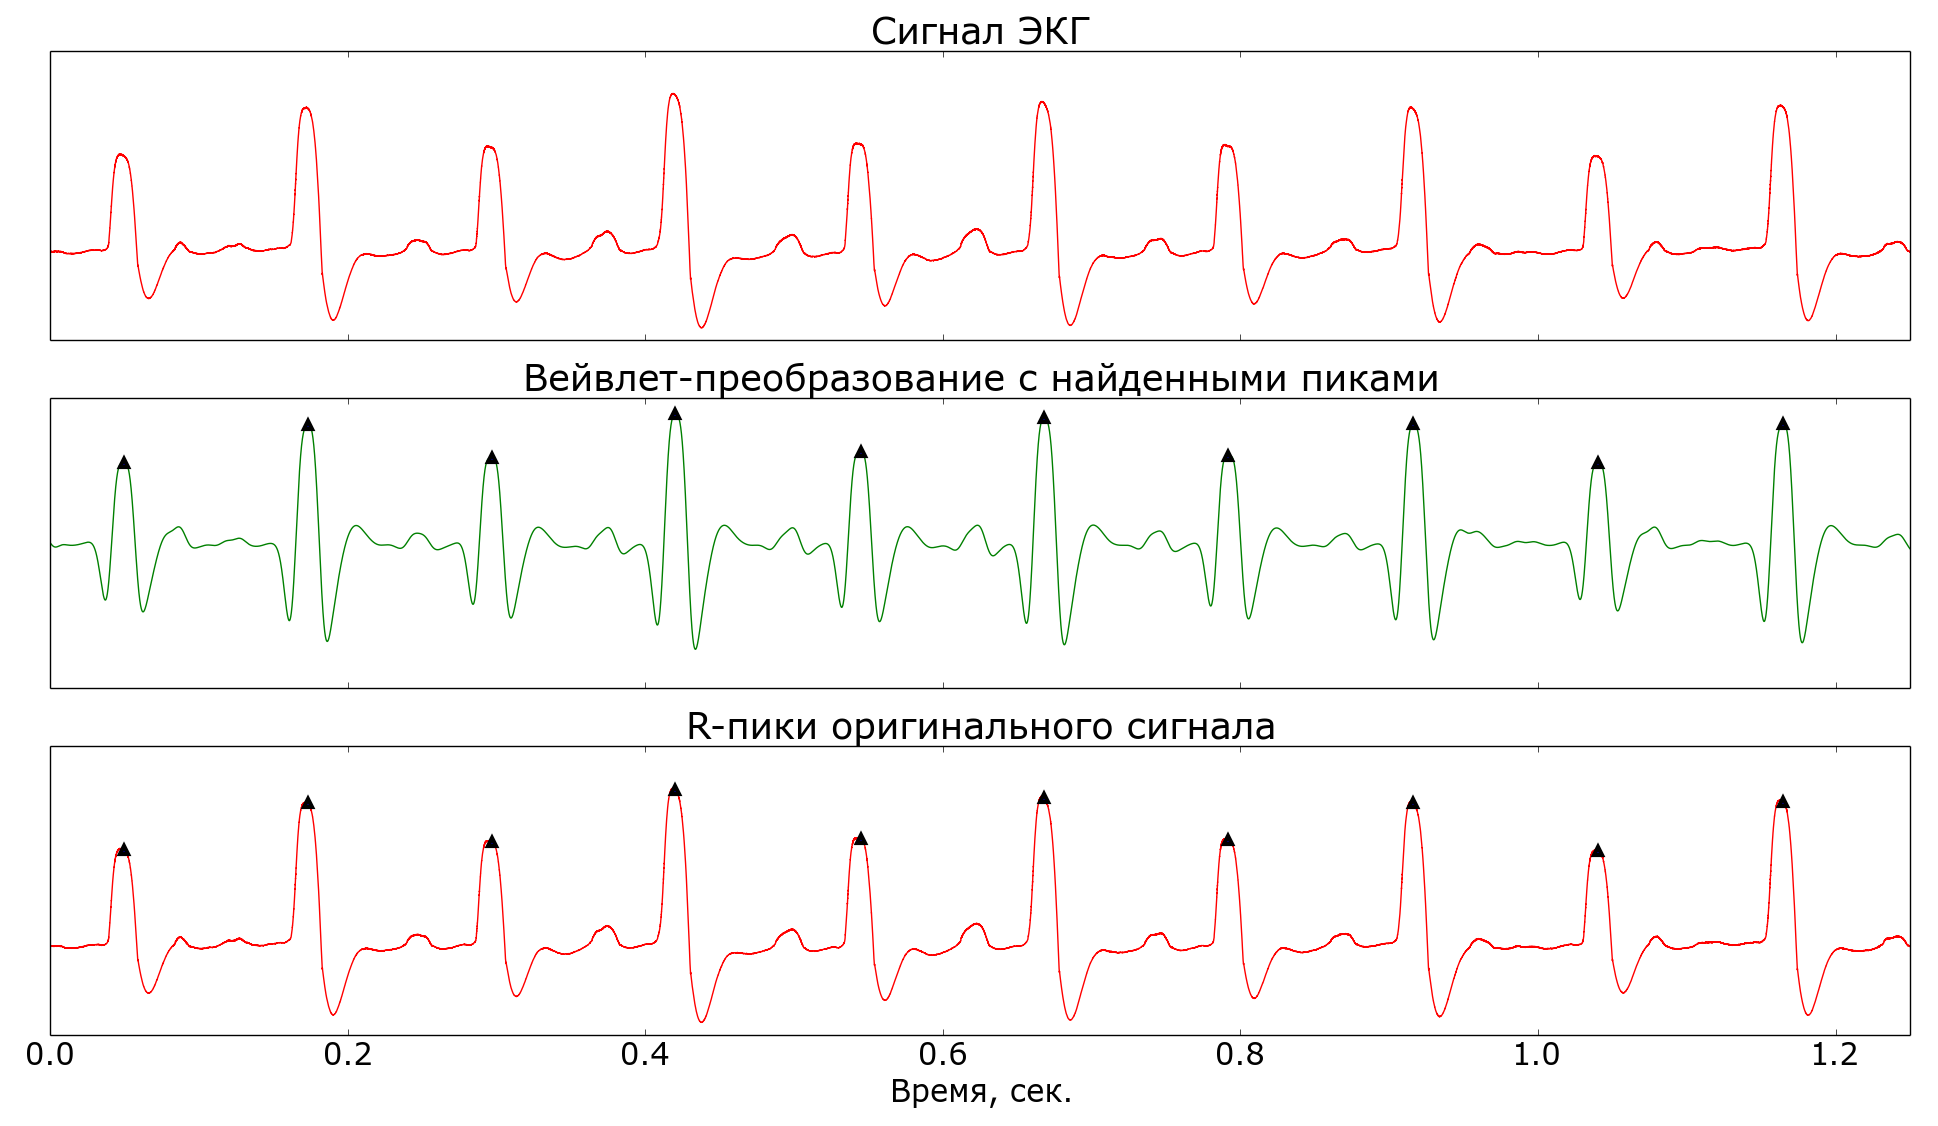
\includegraphics[height = 80mm]{img/record_5_1_R_peaks_detection.png} }
  \caption{Выделение R-пиков}
\end{figure}

Такой метод позволяет корректно выделять кардиоциклы даже из сильно искаженных из-за развития ишемии и проблем аппаратуры сигналов:

\begin{figure}[H]
  \noindent\centering{ 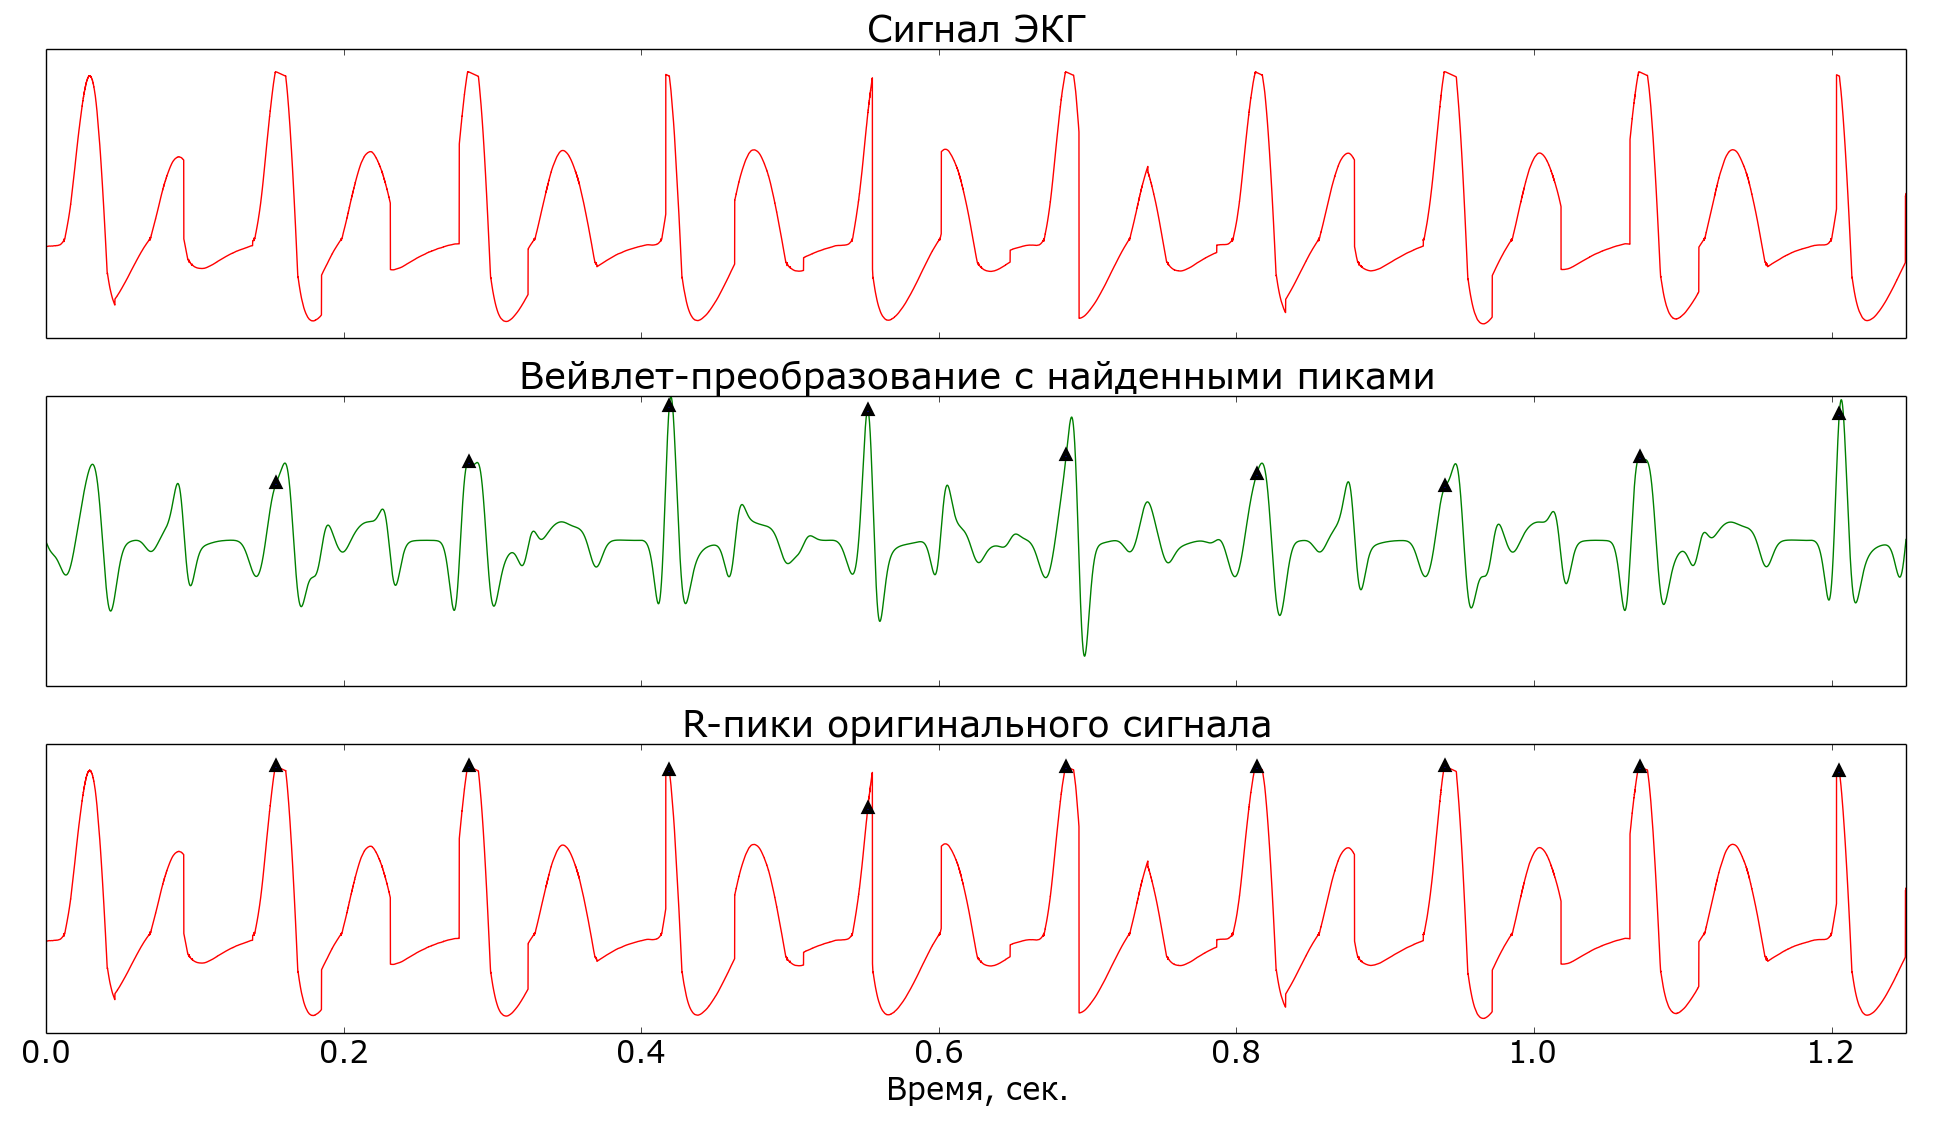
\includegraphics[height = 80mm]{img/record_9_5_R_peaks_detection.png} }
  \caption{Выделение R-пиков из деформированного сигнала}
\end{figure}

Тем не менее, на имеющихся данных кардиоциклы выделяются не всегда корректно. Особенно проблемными являются ЭКГ снятые в процессе развития ишемии:

\begin{figure}[H]
  \noindent\centering{ 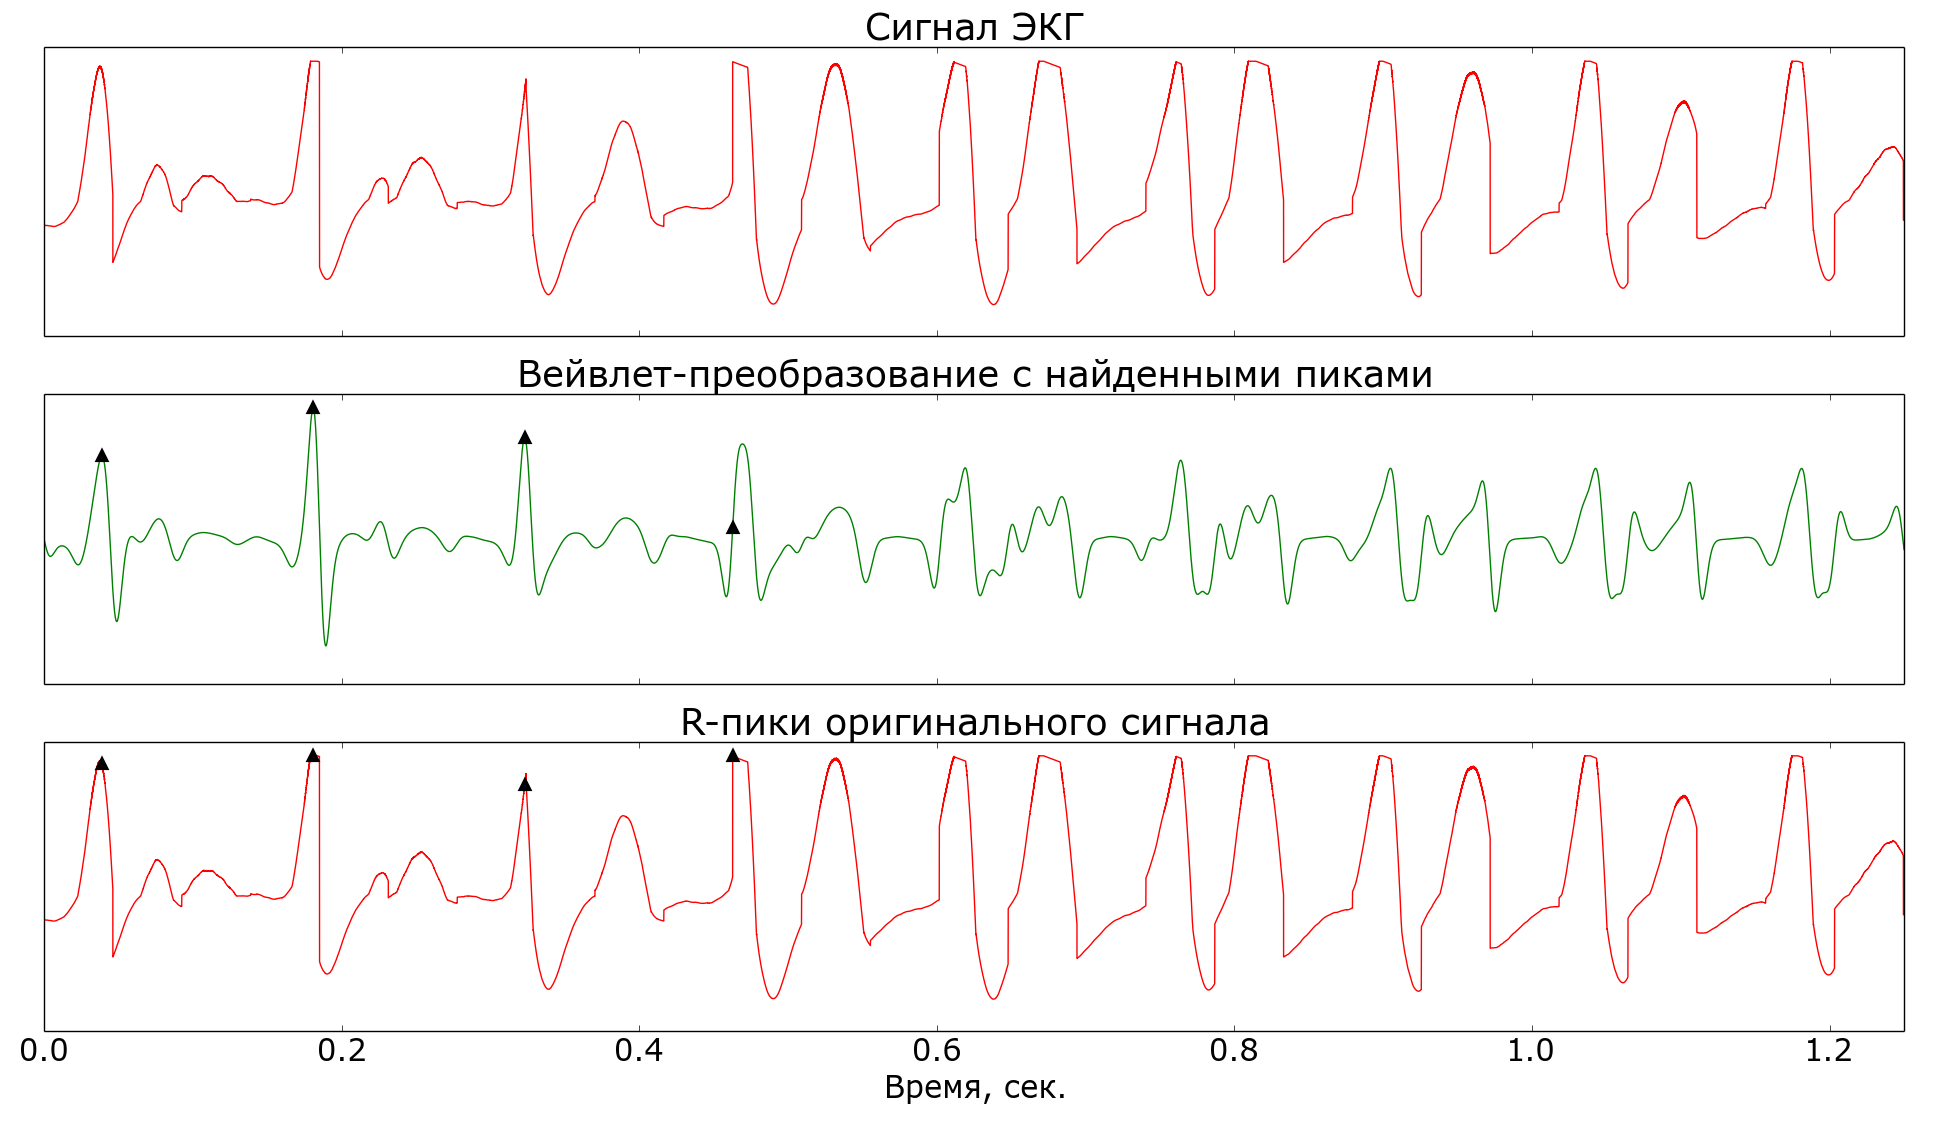
\includegraphics[height = 80mm]{img/record_11_5_R_peaks_detection.png} }
  \caption{Выделение R-пиков из деформированного сигнала}
\end{figure}

В целом, на используемой для классификации части данных, R пики выделяются довольно хорошо. Точность обнаружения составила порядка $90\%$, при чем основная часть пропусков пришлась на записи ЭКГ в ходе развития ишемии. И нет ни одной записи в которой алгоритм не нашел бы ни одного кардиоцикла.

\subsection{Классификация с учетом локальных особенностей АЧХ сигнала}

Используем теперь для классификации систему признаков, описанную в разделе~\ref{sssec:LocalFeaturesTheory}.

У нас имеется способ построения признакового описания, зависящий от трех параметров - ширины окна $\Delta w$, центра окна $w_0$ и количество разбиений интервала частот $n$.

Исследуем как изменяется качество классификации при варировании этих параметров.

Для начала фиксируем ширину окна $\Delta w = 0.4$ и количество разбиений $n=8$ и будем изменять центр окна в интервале $[0, 1]$ с шагом $0.025$:

\begin{figure}[H]
    \begin{center}
        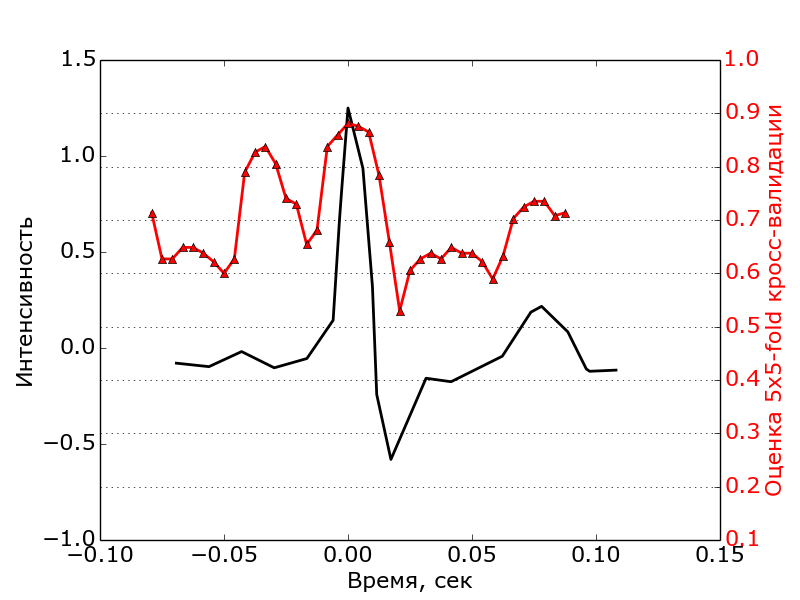
\includegraphics[width=105mm]{img/CV_on_window_center.png}
    \end{center}
    \caption{Зависимость оценки $5\times5 fold$ кросс-валидации от центра окна (ширина окна $\Delta w = 0.4$, количество разбиений $n=8$)}
\end{figure}

На графике видно, что качество классификации имеет явно выраженные пики на участках кардиоцикла, соответствующих зубцам ЭКГ.

Так же заметим, что наилучшее качество классификации достигается на участке, соответствующем R пику кардиограммы.

Фиксируем центр окна в точке $w_0 = 0$ и будем варировать ширину окна:

\begin{figure}[H]
    \begin{center}
        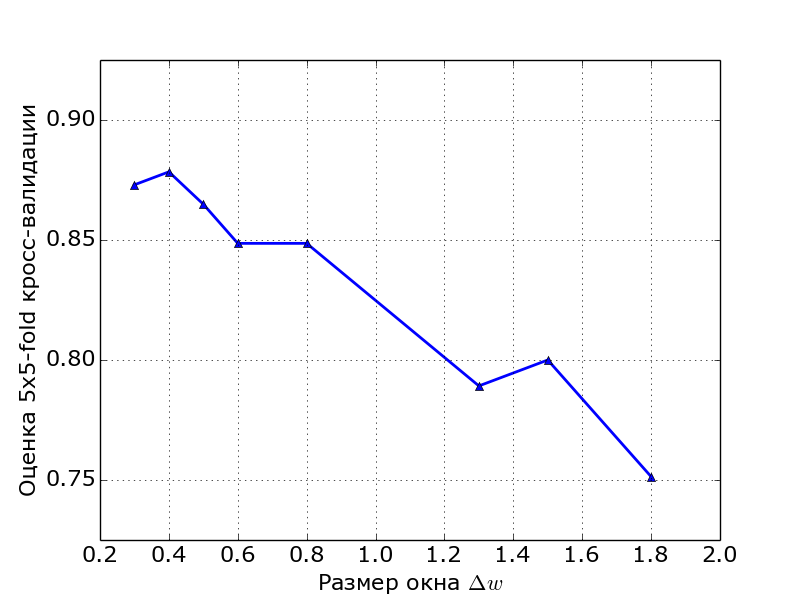
\includegraphics[width=105mm]{img/CV_on_window_size.png}
    \end{center}
    \caption{Зависимость оценки от ширины окна, количество разбиений $n=8$}
\end{figure}

Из графика видно, что максимум качества классификации достигается с шириной окна раной $\Delta w = 0.4$. Это может объясняться тем , что при более широком окне в него попадают другие участки ЭКГ, на которых признаки выражены не так явно. При уменьшении же окна изменяется разрешающая способность оконного преобразования Фурье и плотности интенсивности Фурье-образа на близких частотах становятся неразличимы.

Фиксируем теперь центр и ширину окна и будем варировать количество отрезков разбиения частотного интервала:

\begin{figure}[h]
    \begin{center}
        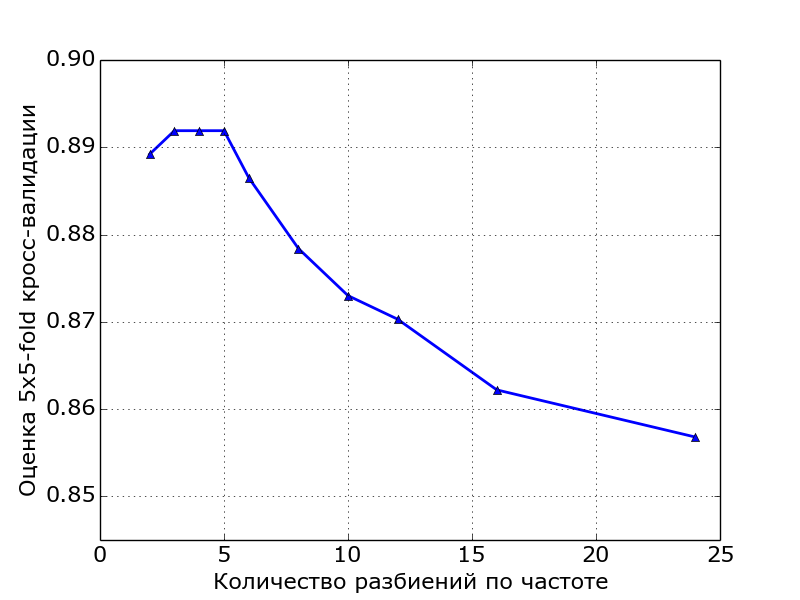
\includegraphics[width=105mm]{img/CV_on_fq_divisions.png}
    \end{center}
    \caption{Зависимость от количества разбиений, ширина окна $\Delta w = 0.4$}
\end{figure}

\subsection{Сравнение классификатора с использованием локальных особенностей и без}

Оценки $5\times5 fold$ кросс-валидации:
\\~\\
\begin{tabular}{|l|c|}
    \hline
    Весь сигнал & $75.7\%$ \\
    \hline
    Окно размером $\Delta w = 0.4$ с центром в R пике & $89.1\%$\\
    \hline
\end{tabular}
\\~\\
ROC-кривые:

\begin{figure}[H]
    \begin{center}
        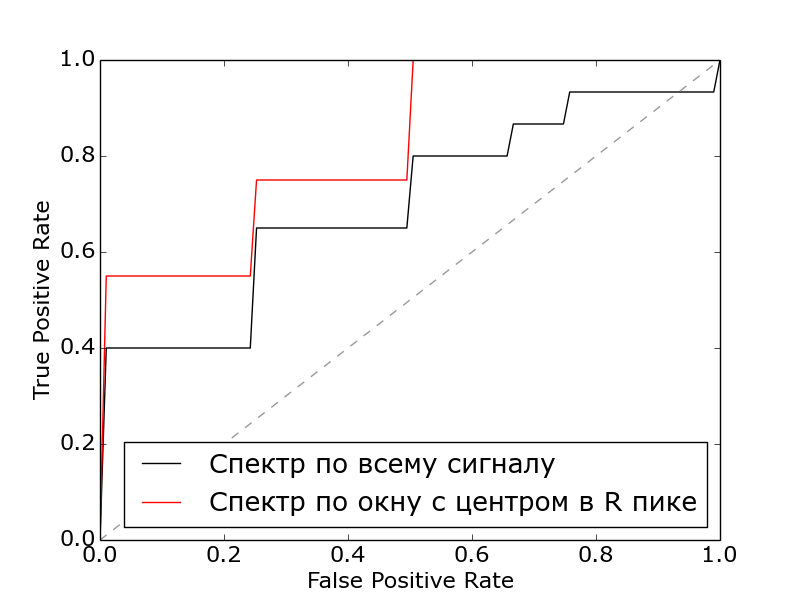
\includegraphics[width=105mm]{img/old_vs_new_roc.png}
    \end{center}
    \caption{Сравнение ROC кривых}
\end{figure}

Из приведенного сравнения видно, что учет локальных особенностей АЧХ сигнала позволяет повысить качество классификации.

\newpage

\section{Заключение}

В данной работе получены следующие результаты:
\begin{itemize}
    \item Исследована задача ранней диагностики ишемической болезни по электрокардиограмме сверхвысокого разрешения. 
    \item Разработан метод диагностики ишемической болезни по данным ЭКГ высокого разрешения, основанный на локализации амплитудно-частотной характеристики ЭКГ-сигнала. 
    \item Экспериментально показано, что локализация позволяет повысить качество диагностики с $75\%$ до $89\%$
\end{itemize}
\newpage
\bibliography{ms_bibliography}
\end{document} 